%%%%%%%%%%%%%%%%%%%%%%%%%%%%%%%%%%%%%%%%%
% Arsclassica Article
% LaTeX Template
% Version 1.1 (1/8/17)
%
% This template has been downloaded from:
% http://www.LaTeXTemplates.com
%
% Original author:
% Lorenzo Pantieri (http://www.lorenzopantieri.net) with extensive modifications by:
% Vel (vel@latextemplates.com)
%
% License:
% CC BY-NC-SA 3.0 (http://creativecommons.org/licenses/by-nc-sa/3.0/)
%
%%%%%%%%%%%%%%%%%%%%%%%%%%%%%%%%%%%%%%%%%

%----------------------------------------------------------------------------------------
%	PACKAGES AND OTHER DOCUMENT CONFIGURATIONS
%----------------------------------------------------------------------------------------

\documentclass[
12pt, % Main document font size
a4paper, % Paper type, use 'letterpaper' for US Letter paper
oneside, % One page layout (no page indentation)
headinclude,footinclude, % Extra spacing for the header and footer
BCOR5mm, % Binding correction
german]{article}


\usepackage[onehalfspacing]{setspace}
\usepackage{mathtools}
\usepackage[export]{adjustbox}
\usepackage{babel,varioref}
\addto\extrasgerman{% page 5 of varioref's manual
  \renewcommand\reftextfaceafter{auf der n{\"a}chsten Seite}%
  \renewcommand\reftextafter {auf der n{\"a}chsten Seite}%
  \renewcommand\reftextfacebefore{auf der vorherigen Seite}%
  \renewcommand\reftextbefore {auf der vorherigen Seite}%
  \renewcommand\reftextcurrent {auf dieser Seite}%
}
\usepackage{listings}
\usepackage{float}
\usepackage{changepage}
%%%%%%%%%%%%%%%%%%%%%%%%%%%%%%%%%%%%%%%%%
% Arsclassica Article
% Structure Specification File
%
% This file has been downloaded from:
% http://www.LaTeXTemplates.com
%
% Original author:
% Lorenzo Pantieri (http://www.lorenzopantieri.net) with extensive modifications by:
% Vel (vel@latextemplates.com)
%
% License:
% CC BY-NC-SA 3.0 (http://creativecommons.org/licenses/by-nc-sa/3.0/)
%
%%%%%%%%%%%%%%%%%%%%%%%%%%%%%%%%%%%%%%%%%

%----------------------------------------------------------------------------------------
%	REQUIRED PACKAGES
%----------------------------------------------------------------------------------------

\usepackage[
nochapters, % Turn off chapters since this is an article        
beramono, % Use the Bera Mono font for monospaced text (\texttt)
eulermath,% Use the Euler font for mathematics
pdfspacing, % Makes use of pdftex’ letter spacing capabilities via the microtype package
dottedtoc % Dotted lines leading to the page numbers in the table of contents
]{classicthesis} % The layout is based on the Classic Thesis style

\usepackage{arsclassica} % Modifies the Classic Thesis package

\usepackage[T1]{fontenc} % Use 8-bit encoding that has 256 glyphs

\usepackage[utf8]{inputenc} % Required for including letters with accents

\usepackage{graphicx} % Required for including images
\graphicspath{{Figures/}} % Set the default folder for images

\usepackage{enumitem} % Required for manipulating the whitespace between and within lists

\usepackage{lipsum} % Used for inserting dummy 'Lorem ipsum' text into the template

\usepackage{subcaption} % Required for creating figures with multiple parts (subfigures)

\usepackage{amsmath,amssymb,amsthm} % For including math equations, theorems, symbols, etc

%\usepackage{varioref} % More descriptive referencing

%----------------------------------------------------------------------------------------
%	THEOREM STYLES
%---------------------------------------------------------------------------------------

\theoremstyle{definition} % Define theorem styles here based on the definition style (used for definitions and examples)
\newtheorem{definition}{Definition}

\theoremstyle{plain} % Define theorem styles here based on the plain style (used for theorems, lemmas, propositions)
\newtheorem{theorem}{Theorem}

\theoremstyle{remark} % Define theorem styles here based on the remark style (used for remarks and notes)

%----------------------------------------------------------------------------------------
%	HYPERLINKS
%---------------------------------------------------------------------------------------

\hypersetup{
%draft, % Uncomment to remove all links (useful for printing in black and white)
colorlinks=true, breaklinks=true, bookmarks=true,bookmarksnumbered,
urlcolor=webbrown, linkcolor=RoyalBlue, citecolor=webgreen, % Link colors
pdftitle={}, % PDF title
pdfauthor={\textcopyright}, % PDF Author
pdfsubject={}, % PDF Subject
pdfkeywords={}, % PDF Keywords
pdfcreator={pdfLaTeX}, % PDF Creator
pdfproducer={LaTeX with hyperref and ClassicThesis} % PDF producer
} % Include the structure.tex file which specified the document structure and layout

\hyphenation{Fortran hy-phen-ation} % Specify custom hyphenation points in words with dashes where you would like hyphenation to occur, or alternatively, don't put any dashes in a word to stop hyphenation altogether

%----------------------------------------------------------------------------------------
%	TITLE AND AUTHOR(S)
%----------------------------------------------------------------------------------------

\title{\normalfont\spacedallcaps{Attack face obfuscation with deep learning using convolution neural networks}} % The article title

%\subtitle{Subtitle} % Uncomment to display a subtitle
\author{Antonio Galeazzi (inf102867@fh-wedel.de) \\ und \\ Till Hildebrandt (inf102835@fh-wedel.de)}

\date{\today} % An optional date to appear under the author(s)

%----------------------------------------------------------------------------------------

\usepackage[font=small,labelfont=bf]{caption}
\begin{document}\selectlanguage{german}

%----------------------------------------------------------------------------------------
%	HEADERS
%----------------------------------------------------------------------------------------

\makeatletter
\renewcommand\paragraph{\@startsection{paragraph}{4}{\z@}%
            {-2.5ex\@plus -1ex \@minus -.25ex}%
            {1.25ex \@plus .25ex}%
            {\normalfont\normalsize\bfseries}}
\makeatother

\makeatletter
\renewcommand{\@seccntformat}[1]{%
  \ifcsname format#1\endcsname
    \csname format#1\endcsname
  \else
    \csname the#1\endcsname\quad
  \fi
}
\makeatother
%
%\newcommand{\formatsection}{\thesection: }
%\newcommand{\formatsubsection}{\thesubsection: } % just for example
%\newcommand{\formatsubsubsection}{\thesubsubsection: } % just for example

\setcounter{secnumdepth}{4} % how many sectioning levels to assign numbers to
\setcounter{tocdepth}{4}    % how many sectioning levels to show in ToC
\renewcommand{\sectionmark}[1]{\markright{\spacedlowsmallcaps{#1}}} % The header for all pages (oneside) or for even pages (twoside)

\renewcommand{\lstlistingname}{Code-Auszug}%
\lstset{basicstyle=\ttfamily,
  showstringspaces=false,
  commentstyle=\color{red},
  keywordstyle=\color{blue}
}
\lehead{\mbox{\llap{\small\thepage\kern1em\color{halfgray} \vline}\color{halfgray}\hspace{0.5em}\rightmark\hfil}} % The header style
%\pagestyle{scrheadings} % Enable the headers specified in this block

\captionsetup[figure]{labelfont={bf},name={Abbildung}}
\newcommand\amusingversion[2]{%
    \vrefpagenum\firstnum{#1}%
    \vrefpagenum\secondnum{#2}%
    \ifthenelse{\equal\firstnum\secondnum}%
    {s of \ref{#1} and \ref{#2} \vpageref{#1}}%
    { of \ref{#1} \vpageref{#1} and of \ref{#2} \vpageref{#2}}%
    }


%----------------------------------------------------------------------------------------
%	TABLE OF CONTENTS & LISTS OF FIGURES AND TABLES
%----------------------------------------------------------------------------------------

\maketitle % Print the title/author/date block

\setcounter{tocdepth}{2} % Set the depth of the table of contents to show sections and subsections only

\clearpage

\tableofcontents % Print the table of contents

%----------------------------------------------------------------------------------------

\newpage % Start the article content on the second page, remove this if you have a longer abstract that goes onto the second page

%----------------------------------------------------------------------------------------
%	INTRODUCTION
%----------------------------------------------------------------------------------------
\section{Einleitung}

Machine Learning stellt einen Aspekt der künstlichen Intelligenz dar, der in der vergangenen Zeit an immer größerer
Bedeutung gewonnen hat. In diesem Kontext ist insbesondere das Deep Learning hevorzuheben, das wiederum einen Teilbereich
des Machine Learnings darstellt. Dessen Popularität lässt sich zum Einen damit erklären, dass es die Geschwindigkeit und
Reife heutiger Prozessoren (CPU/GPU/TPU\footnote{Wikipedia, Tensor Processing Unit.\newline
(https://de.wikipedia.org/wiki/Tensor\_Processing\_Unit)}/FPGA\footnote{Wikipedia, Field Programmable Gate Array.\newline
(https://de.wikipedia.org/wiki/Field\_Programmable\_Gate\_Array)})
zulässt Ergebnisse in akzeptabler Zeit zu erzielen und zum Anderen damit, dass durch das stetige Anwachsen der durchs Internet
erzeugten Daten, genug Material zur Verfügung steht, mit dem gearbeitet werden kann. Besonders im Kontext von Bilderkennungen
und Klassifizierungsproblemen sind Techniken des Machine Learnings kaum noch wegzudenken.

In bildgebenden Medien, Videos wie Fotos, werden Gesichter von Menschen verfälscht, um deren Identität unkenntlich
zu machen.\footnote{Andrew Senior, Protecting Privacy in Video Surveillance, S 130 ff.\label{fn:protecting_privacy}}
Diese Technologien werden von
öffentlichen Medien, wie Privatpersonen verwendet. In der Vergangenheit
gab es den Fall eines Kinderschänders, der verfälschte Gesichtsbilder von sich veröffentlichte. Er verwendete dabei
ein Verfahren, das Pixel um einen zentralen Punkt zu einer Spirale rotiert. Behörden war es damals möglich, diese
Form der Gesichtsverfälschung, der Informationsverlust im Vergleich zu den Verfahren, die in dieser Arbeit behandelt
werden, gering ist, aufzuheben und das Gesicht weitgehends wiederherzustellen.
\footnote{Wikipedia, ``Christopher Paul Neil''.\newline(https://en.wikipedia.org/wiki/Christopher\_Paul\_Neil)}
Motiviert unter anderem dadurch,
stellt diese Arbeit eine Grundlagenanalyse dar, in wie weit CNNs dafür verwendet werden können sehr viel verbreitetere,
aber destruktive Obfuscation-Verfahren anzugreifen.

Maßgablich kommen beim Verfälschen zwei Verfahren zum Einsatz\textsuperscript{\ref{fn:protecting_privacy}}:
``Weichzeichnen'' (Gaussian Blur)\footnote{Wikipedia, Gaussian Blur.\newline(https://en.wikipedia.org/wiki/Gaussian\_blur)}
 und ``Verpixelung'' (Pixelization)\footnote{Wikipedia, Pixelization.\newline(https://en.wikipedia.org/wiki/Pixelization)\label{label:pixelization}}.


\subsection{Weichzeichnen}
Der gaußscher Weichzeichner oder Gaussian smoothing, beschreibt ein Verfahren, mit dem der Kontrast von Bildern
verrinngert wird. Damit wird der Verlust von Detailinformationen erreicht. Die mathematische Formel, nach der die
Transformation funktioniert, lautet:

\parskip\baselineskip

\begin{figure}[h]
    \centering
    \(G(x) = \frac{1}{\sqrt{2 \pi \sigma^2}} e^{-\frac{x^2}{2 \sigma^2}}\)
    \caption{Gleichung der gausschen Weichzeichnung zweier Dimensionen.}
    \label{fig:func-blur}
\end{figure}


\par
\par

\textit{x} und \textit{y} beschreiben die Distanz zum Ursprung der jeweiligen Achse, \textit{\(\sigma\)} ist ein Parameter der Funktion, der
beschreibt wie sehr die Weichzeichnung streut (siehe Abbildung \space \vref*{fig:gaussianBlur}).
Der Formel kann man entnehmen, dass die
Farbinformationen benachbarter Pixel in das Ergebnis des aktuell zu berechnenden Pixels miteinfließen. Hier werden
die Informationen verschiedener Pixel auf den selben Wertebereich eines Pixels abgebildet. Der dadurch entstehende
Informationsverlust ist irreversibel.

\captionsetup[subfigure]{labelformat=empty, labelsep=none}
\begin{figure}[h]
    \centering
    \begin{subfigure}{0.3\textwidth}
        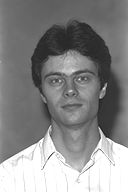
\includegraphics[width=0.9\textwidth]{introduction_blur_original}
        \caption{\small Original}
    \end{subfigure}
    \begin{subfigure}{0.3\textwidth}
        
\includegraphics[width=0.9\textwidth]{introduction_blur_sigma_3}
        \caption{\small \(\sigma = 3\)}
    \end{subfigure}
    \begin{subfigure}{0.3\textwidth}
        
\includegraphics[width=0.9\textwidth]{introduction_blur_sigma_6}
        \caption{\small \(\sigma = 6\)}
    \end{subfigure}

    \caption{Vergleichsbild Weichzeichnen mit verschiedenen Parametern.}
    \label{fig:gaussianBlur}
\end{figure}

\subsection{Verpixelung}
Auch Mosaic-Verfahren, meint eine Menge an Verfahren, die die Auflösung von Bildern oder Bereiche derer künstlich
verringern, um Detailinformationen zu verbergen. Hierfür wird der unkenntlich zu machende Bereich in gleichmäßige
Unterbereiche aufgeteilt und deren resultierender Farbwert aus den Pixeln des Ursprungsbildes gemittelt. Bei dieser
Verfahrensfamilie gibt es eine Vielzahl an Variationen, die sich in Größe und Form der Unterbereiche und dem genauen
Algorithmus, der verwendet wird, um die Unterbereiche unkenntlich zu machen.

\begin{figure}[h]
    \centering
    \begin{subfigure}{0.3\textwidth}
        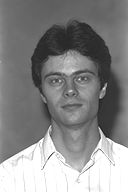
\includegraphics[width=0.9\textwidth]{introduction_mosaic_original}
        \caption{\small Original}
    \end{subfigure}
    \begin{subfigure}{0.3\textwidth}
        
\includegraphics[width=0.9\textwidth]{introduction_mosaic_5}
        \caption{\small Kantenlänge 5px}
    \end{subfigure}
    \begin{subfigure}{0.3\textwidth}
        
\includegraphics[width=0.9\textwidth]{introduction_mosaic_10}
        \caption{\small Kantenlänge 10px}
    \end{subfigure}

    \caption{Vergleichsbild Weichzeichnen mit verschiedenen Kantenlängen.}
    \label{fig:pixelization}
\end{figure}

Der in diesem Verfahren betrachtete Parameter (siehe Abbildung \space \vref*{fig:pixelization}), entspricht der Kantenlänge der
resultierenden verpixelten Unterbereiche.


\section{Datenquellen und Aufbereitung}

Als grundlegende Datenquelle wurden die
\textit{color FERET Database}\footnote{NIST, color FERET Database.\newline(https://www.nist.gov/itl/iad/image-group/color-feret-database)\label{footnote:color-feret}},
die von dem National Institute of Standards and Technology veröffentlicht wurde, und die
Datenbank \textit{FaceScrub} von \textit{vintage}\footnote{vision \& interaction groupe, FaceScrub.\newline(http://vintage.winklerbros.net/facescrub.html\label{footnote:face-scrub}} verwendet.

Die \textit{color FERET Database}\textsuperscript{\ref{footnote:color-feret}} umfasst 11.338 Gesichtsbilder von 1.208 Menschen, die in einer kontrollierten Umgebung augenommen worden sind, und
hält neben Metadaten über Pose, Geschlecht, Ethnie und Alter auch weiterführende Daten bereit wie Augenposition und
Kamerawinkel. Die Daten liegen im Portable Pixmap Format RGB- und im Graustufenformat homogen in einer vor Maximalauflösung von \textit{512 \(\times\) 768} Pixeln vor.

Die \textit{FaceScrub}\textsuperscript{\ref{footnote:face-scrub}} Datenbank umfasst über 100.000 Gesichtsbilder von 530 prominenten Menschen, die in einer unkontrollierten Umgebung augenommen worden sind und stellt keine
weiteren Metadaten bereit. Die Daten liegen im JPEG-Format in einer vor Maximalauflösung von \textit{512 \(\times\) 768} Pixeln vor.


Um trotz der vergleichsweise geringen Datenmenge. Vergleichbare Projekte\footnote{Richard McPherson, Rezar Shokri, Vitali Shmatikov, Defeating Image Obfuscation with Deep Learning.\newline(https://arxiv.org/pdf/1609.00408.pdf)}
verwenden hingegen 60.000 bis 300.000 Bilder, interpretierbare Ergebnisse erzielen zu können, beschränkt sich diese Arbeit auf
die Verwendung möglichst homogener Bilder unterschiedlicher Personen. Von besonderem Interesse ist hierbei die Pose des
Abgebildeten. Die Datenbank unterscheidet Frontal- und Profilbilder sowie Bilder, in denen der Kopf um einen bestimmten
Winkel gedreht ist. Als grundlegenden Datensatz wurde sich für die Frontalbilder entschieden, da diese mit 2.722 Bilder
von 994 Personen den großten Teildatensatz ausmachen.

Die benötigten Testdatensätze wurde mithilfe von ImageMagick\footnote{ImageMagick Studio LLC, ImageMagick.\newline(https://www.imagemagick.org/)} in Version 6.8. aufbereitet. Um die Komplexität der
Problemstellung weiter zu reduzieren, wurden die Bilder grauskaliert und auf 12,5\% der Ursprungsgröße skaliert, sodass
die Trainigsdaten noch eine Auflösung von 64 \(\times\) 96 Pixeln haben. Es wurden vier unterschiedliche Testdatensätze mit
folgenden CLI-Befehlen generiert \footnote{Das folgende BASH-Skript scripts/create\_images.sh erzeugt die
Testdaten. Notwendig hierfür sind die Pakete \textit{imagemagick} und \textit{imagemagick-doc}.}:


\begin{minipage}{\linewidth}

\begin{lstlisting}[language=bash,caption={convert - Synopsis}]
convert [input-options] input-file [output-options] output-file
\end{lstlisting}

\begin{lstlisting}[language=bash,caption={Testdatenerstellung - Graustufen}]
#!/bin/bash

# every call scales the input image down to 12.5% of its
# original size and grayscales it.

# convert test data:  gaussian-blur (sigma = 3)
convert <input_file.ppm> \
    -set colorspace Gray \  # grayscale durch
    -separate \             # separates (RGB)
    -average \              # Mittel
    -scale 12.5\% \         # Skalierung auf 96px x 64px
    -gaussian-blur 0x3 \    # blur
    <output_file.pgm>; mv <output_file.pgm> <output_file.ppm>

# convert test data:  gaussian-blur (sigma = 6)
convert <input_file.ppm> \
    -set colorspace Gray \
    -separate \
    -average \
    -scale 12.5\% \
    -gaussian-blur 0x6 \
    <output_file.pgm>; mv <output_file.pgm> <output_file.ppm>

# convert test data:  pixelization (edge length = 5px)
convert <input_file.ppm> \
    -set colorspace Gray \
    -separate \
    -average \
    -scale 12.5\% \
    -scale $(( bc <<< "scale=100;100/5" ))\% \
    -scale 500\% \
    <output_file.pgm>; mv <output_file.pgm> <output_file.ppm>

# convert test data:  pixelization (edge length = 10px)
convert <input_file.ppm> \
    -set colorspace Gray \
    -separate \
    -average \
    -scale 12.5\% \
    -scale $(( bc <<< "scale=100;100/10" ))\% \
    -scale 1000\% \
    <output_file.pgm>; mv <output_file.pgm> <output_file.ppm>
\end{lstlisting}
\end{minipage}

\section{Neuronale Netze}

Die nachfolgenden Ausführungen und Graphiken zum Schaffen eines grundlegenden Verständnisses des Machine Learnings
basieren im wesentlichen auf dem E-Book ``Neural Networks and Deep Learning''\footnote{Michael Nielsen, Neural Networks and Deep Learning.\newline
(http://neuralnetworksanddeeplearning.com/index.html)}.

Im Rahmen des maschinellen Lernens stellen die neuronalen Netze einen elementaren Ansatz dar,
der in vielen weiteren Modellen Verwendung findet. Neuronale Netze wie das maschinelle Lernen an sich
stellen eine andere Herangehensweise dar, als die klassischer, deterministischer Algorithmen.

Anstatt dem System eine eindeutige Abfolge von Anweisungen mitzuteilen, um eine konkrete Problemstellung
zu lösen, definiert man ein Modell und konfrontiert dieses mit verschiedenen Beispielen - die Beispiele
sind dabei Tupel aus Eingangsgröße und erwarteter Ausgangsgröße. Die Dimensionen von Eingangs- und Ausgangsgröße
können sich dabei gleichen, müssen es aber nicht. So können als Eingabe Bilder dienen und als
Ausgaben konkrete Klassen, um beispielsweise Hunde von Katzen unterscheiden zu können.

Anstatt nun algorithmisch zu definieren, was einen Hund von einer Katze unterscheidet, überlässt man es dem zuvor
erstellten Modell anhand der gegebenen Eingaben und erwarteten Ausgaben, eigenständig Regeln abzuleiten, um mit
dessen Hilfe auch unbekannte Eingaben klassifizieren zu können.

Dieser Ansatz wird als \textit{Soft Computing} bezeichnet.

\subsection{Perzeptron}

Als elementaren Bestandteil eines neuronalen Netzes dient das \textit{Perzeptron} - dieses stellt
die kleinste Einheit eines neuronalen Netztes dar und wird auch als ``künstliches Neuron'' bezeichnet.

Grundsätzlich akzeptiert ein Neuron einen beliebig großen Input bestehend aus Features \textit{x1, x2, ..., xn} und
berechnet daraus ein Ergebnis.

\begin{figure}[h]
    \centering
    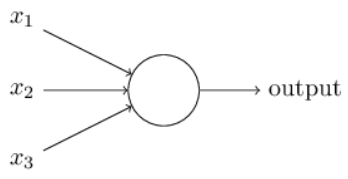
\includegraphics[width=0.5\textwidth]{docu_img_01}
    \caption{Perzeptron}
    \label{fig:perzeptron}
\end{figure}

Im gezeigten Bild ist beispielsweise ein Neuron dargestellt, das drei Inputgrößen akzeptiert und daraus einen Output
produziert. Um den Output zu berechnen werden Gewichte (\textit{engl. weights}) eingeführt. Ob das Neuron 0 oder 1 als
Output liefert, hängt dann davon ab, ob die gewichtete Summe der Eingangsgrößen einen zu definierenden Schwellwert
überschreitet.

Dies kann anhand des nachfolgenden Bilds verdeutlicht werden:

\begin{figure}[h]
    \centering
    \[ output =
      \begin{cases}
        0 \quad \text{if } \sum \omega_i x_i \leqslant \text{ threshold (Schwellwert)}\\
        1 \quad \text{if } \sum \omega_i x_i > \text{ threshold (Schwellwert)}
      \end{cases}
    \]
    \caption{Berechnung des Outputs.}
    \label{fig:neuron-three-way}
\end{figure}


Dies ist das grundlegende Modell. Grundsätzlich kann man sich das Perzeptron als einen ``Entscheidungs-Unterstützer''
vorstellen, der eine Entscheidung trifft, in dem er konkrete Fakten mit einem bestimmten Gewicht versieht.

Das gezeigte Modell ist augenscheinlich sehr simpel und noch sehr weit von dem entfernt, was man als ein neuronales
Netz bezeichnen würde. Es ist allerdings ohne Weiteres denkbar, das gezeigte Model komplexer zu gestalten, indem
mehrere Perzeptrons miteinander verknüpft werden, so dass beispielsweise das nachfolgende Netzwerk entstehen könnte:

\begin{figure}[h]
    \centering
    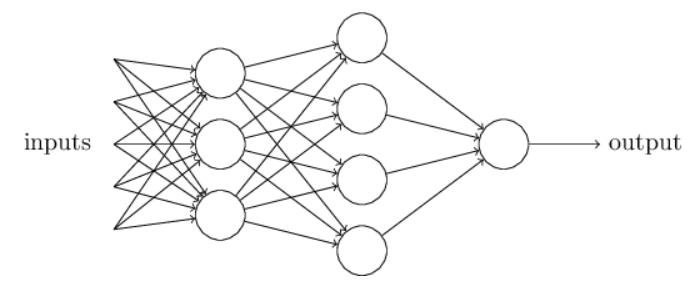
\includegraphics[width=0.5\textwidth]{docu_img_03}
    \caption{Mehrschichtiges neuronales Netz.}
    \label{fig:multi-layer-net}
\end{figure}

In Grafik\textsuperscript{\ref{fig:neuron-three-way}} wurde ein Schwellwert eingeführt, der überschritten werden muss, damit ein Perzeptron
aktiviert wird. Um das Modell zu vereinheitlichen, kann der \textit{Bias} definiert werden, der den
negativen Schwellwert darstellt. Durch diese Maßnahme kann die Aktivierungsfunktion des Perzeptrons dann geschrieben
werden als:

\begin{figure}[h]
    \centering
    \[ output =
          \begin{dcases}
            0 \quad \text{if } \sum \omega \cdot x + b \leq 0 \\
            1 \quad \text{if } \sum \omega \cdot x + b > 0
          \end{dcases}
    \]
    \caption{Berechnung des Outputs bei Verwendung eines Bias.}
    \label{fig:bias-calculation}
\end{figure}

Inhaltlich kann das Bias als ein Maß verstanden werden, aus dem hervorgeht, wie leicht ein Perzeptron aktiviert
werden kann. Nimmt der Bias einen großen Wert an, so kann das Perzeptron einen Wert von 1 annehmen, auch wenn das
Produkt aus den Gewichten und den Eingangsgrößen einen negativen Wert annimmt. Gleiches gilt selbstverständlich auch für
einen kleinen Bias, der zur Folge hat, dass ein Perzeptron träger reagiert.

\subsection{Sigmoid-Neuronen}

Eine Weiterentwicklung des zuvor vorgestellten Modells stellen Sigmoid-Neuronen dar. Diese Weiterentwicklung wird
dann erforderlich, wenn das Anpassen der Gewichte - also letztlich das Lernen - betrachtet wird. Dabei ist das Ziel,
dass eine kleine Anpassung eines Gewichts auch nur eine kleine Änderung des Outputs zur Folge hat. Das zuvor
betrachtete Perzeptron ist lediglich in der Lage 0 oder 1 als Output zu liefern, so dass Änderungen an den Gewichten
keine stetige Änderung des Outputs zur Folge haben, sondern folgenlos bleiben können bis irgendwann ein Sprung von 0
auf 1 oder umgekehrt stattfindet, was wiederum eine große Änderung darstellt.

Die Weiterentwicklung besteht nun in einer Verfeinerung der Aktivierungsfunktion. Anstatt eine Sprungfunktion\textsuperscript{\ref{fig:step-function}} zu
verwenden, die lediglich 0 und 1 als Funktionswert annehmen kann, wird die Sigmoid Funktion\textsuperscript{\ref{fig:sigmoid-function}} eingeführt,
die die folgende Form hat:

\begin{figure}[h]
    \centering
    \[ \sigma(z) \equiv
          \frac{1}{1+e^{-z}}
    \]
    \caption{Sigmoid-Funktion.}
    \label{fig:sigmoid}
\end{figure}

Der entscheidende Unterschied kann an den beiden nachfolgenden Grafiken verdeutlicht werden, die jeweils die Kurve
der entsprechenden Funktion darstellen:

\captionsetup[subfigure]{labelformat=empty, labelsep=none}
\begin{figure}[h]
    \centering
    \begin{subfigure}{0.45\textwidth}
		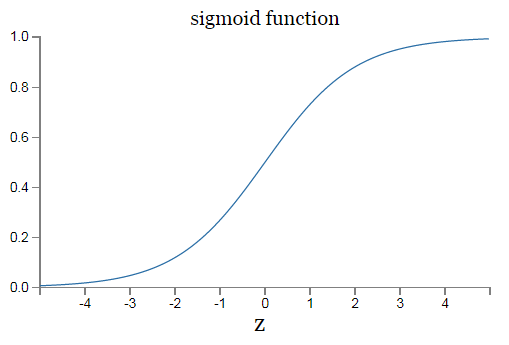
\includegraphics[width=0.9\textwidth]{docu_img_06}
		\caption{\tiny{Sigmoid Funktion.}}
		\label{fig:sigmoid-function}
	\end{subfigure}
    \begin{subfigure}{0.45\textwidth}
		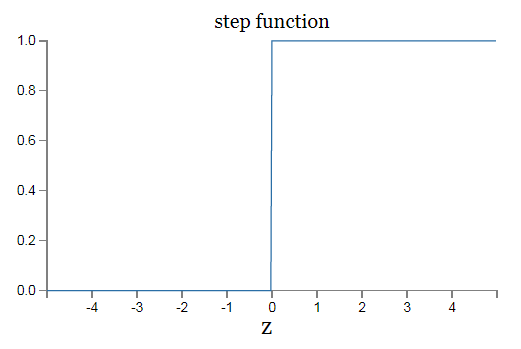
\includegraphics[width=0.9\textwidth]{docu_img_07}
		\caption{\tiny{Step Funktion.}}
		\label{fig:step-function}
	\end{subfigure}

    \caption{Vergleich der Aktivierungsfunktionen \textit{Sigmoid} und \textit{Step-Funktion}}
    \label{fig:activation-functions}
\end{figure}

\subsection{Architektur neuronaler Netze}

Mit diesen Bestandteilen als Ausgangspunkt können nun tatsächlich konkretere Neuronale Netze und deren Architekturen
eingeführt werden. Neuronale Netze bestehen üblicherweise aus mehreren Schichten, den \textit{Layern}. Diese lassen
sich grundsätzlich in drei Kategorien aufteilen: Input, Hidden und Output. Neuronale Netze beinhalten für gewöhnlich
ein Input-Layer und ein Output-Layer sowie dazwischen beliebig viele Hidden-Layer. Die Form der Input- und Output-Layer
ist dabei sehr naheliegend: das Input-Layer hat die gleiche Struktur wie die des Inputs und das Output-Layer hat
entsprechend die gleiche Struktur wie der Output.

Angenommen es sollen Bilder der Größe 28 \(\times\) 28 Pixel klassifiziert werden und es gibt 10 mögliche Klassen, dann besteht das
Input-Layer aus 28 \(\times\) 28 = 784 Neuronen und das Output-Layer aus 10 Neuronen.

Lediglich der Bereich zwischen Input- und Output-Layer - die Hidden-Layer - lässt sich nicht ohne Weiteres aus dem Input
oder dem Output ableiten. Es gibt lediglich Heuristiken, die beim Design der Hidden-Layer angewandt werden können,
allerdings keine konkreten Regeln, die befolgt werden müssen. Diese Struktur kann anhand des nachfolgenden Bilds
verdeutlicht werden, bei dem - um die Übersichtlichkeit zu wahren - das Input-Layer etwas komprimiert dargestellt wird:

\begin{figure}[h]
    \centering
    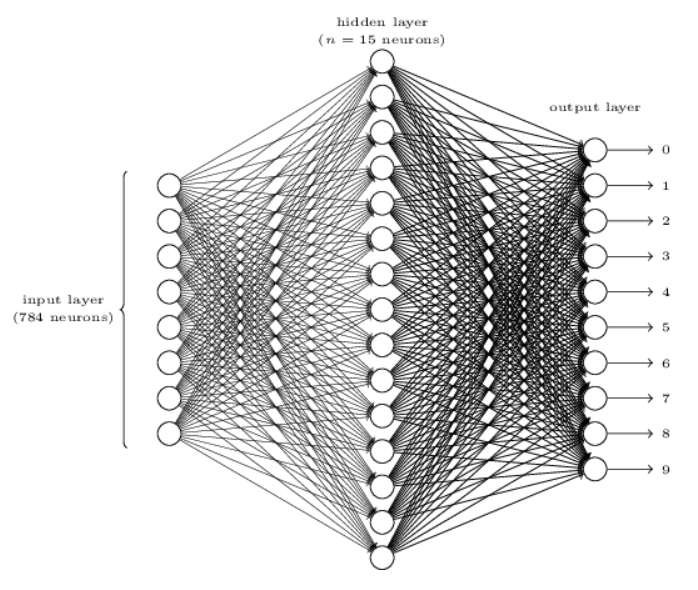
\includegraphics[width=0.9\textwidth]{docu_img_08}
    \caption{Hidden-Layer Darstellung.}
    \label{fig:hidden-layers}
\end{figure}

\subsection{Lernen - Das Anpassen der Gewichte}

Das Lernen stellt den zentralen Ansatz von neuronalen Netzes dar. Eng im Zusammenhang mit dem Lernen steht eine
Kosten-Funktion, die häufig auch als Verlust-Funktion bezeichnet werden kann. Diese stellt letztlich den Fehler zwischen
dem Erwartungswert und dem tatsächlichen Wert, den das neuronale Netz berechnet, dar. Mathematisch betrachtet ist das
grundlegende Prinzip des Lernens diese Funktion zu minimieren, also zu gewährleisten, dass die Abweichungen zwischen
Erwartungswert und tatsächlichem Wert möglichst gering sind. Es sind grundsätzlich viele verschiedene Verlust-Funktionen
denkbar, eine, die jedoch eine breite Verwendeung findet, ist die quadratische Kosten-Funktion - auch als \textit{mean squared
error} (MSE) bezeichnet.

\begin{figure}[h]
    \centering
    \[ C(w, b) \equiv
          \frac{1}{2n}\displaystyle\sum_{x}{\parallel y(x) - a\parallel^2}
    \]
    \caption{Mean Squared Error (MSE).}
    \label{fig:learn-function}
\end{figure}

Dabei beschreiben \textit{w} und \textit{b} die Gewichte bzw. die Bias des neuronalen Netzes und \textit{n} stellt die Anzahl der Trainingsdaten
dar. Der Vektor a beschreibt den Output des Netzes und \textit{\(y(x)\)} stellt den Erwartungswert zu einem Input \textit{x} dar.
Das Ziel besteht nun darin, die Gewichte und Bias so zu manipulieren, dass die gezeigte Funktion einen möglichst kleinen
Wert annimmt.

\subsection{Gradientenabstieg (Gradient Descent)}

Um die soeben eingeführte Kostenfunktion zu minimieren, wird ein Verfahren verwendet, das als Gradientenabstieg (\textit{engl.
gradient descent}) bezeichnet wird. Neben dem hier vorgestellten Verfahren existieren noch viele weitere Methoden, die
zur Lösung dieses Optimierungs- bzw. Minimierungsproblems verwendet werden können.
Zur Veranschaulichung des Problems soll nun eine Funktion zweier Variablen, die minimiert werden soll, betrachtet werden.

\begin{figure}[h]
    \centering
    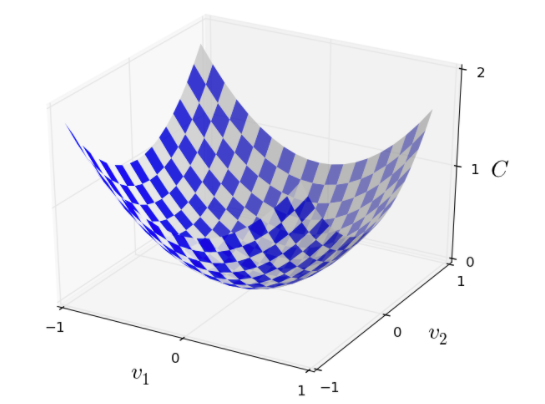
\includegraphics[width=0.9\textwidth]{docu_img_17}
    \caption{Darstellung des Gradientenabstieg bei einer Funktion in Abhängigkeit von zwei Variablen.}
    \label{fig:gradient-decent-3d}
\end{figure}

Dieses Problem könnte selbstverständlich durch Verfahren der Analysis gelöst werden. In der Realität ist die Anzahl der
Variablen jedoch um ein Vielfaches höher, sodass diese Verfahren nicht mehr effizient angewandt werden können.

Zur Visualisierung der grundlegenden Idee des Gradientenabstiegs kann sich ein Ball vorgestellt werden, der sich abwärts
in Richtung eines Tals bewegt. Bewegt man den Ball etwas in Richtung \textit{v1} und etwas in Richtung \textit{v2}
so gilt für den Funktionswert \textit{C}:

\begin{figure}[h]
    \centering
    \[ \Delta C \approx
          \frac{\delta C}{\delta v_1} \Delta v_1 + \frac{\delta C}{\delta v_2} \Delta v_2
    \]
    \caption{Veränderung des Funktionswerts.}
    \label{fig:gradient-decent-definition}
\end{figure}

Der Gradient wird dann folgendermaßen definiert:

\begin{figure}[h]
    \centering
    \[ \nabla C \equiv
        (\frac{\delta C}{\delta v_1},\frac{\delta C}{\delta v_2})^T
    \]
    \caption{Definition des Gradienten}
    \label{fig:gradient-decent-definition-2}
\end{figure}

Durch die Verwendung dieses mathematischen Objekts kann die vorherige Gleichung\textsuperscript{\ref{fig:gradient-decent-definition}} formuliert werden als:

\begin{figure}[h]
    \centering
    \[ \delta C \approx
        \nabla C \cdot \delta v
    \]
    \caption{Veränderung des Funktionswerts durch Gradienten ausgedrückt}
    \label{fig:gradient-decent-definition-3}
\end{figure}

Wird die Veränderung der Variablen (Gewichte) nun so gewählt, dass sie dem Inversen des Gradienten multipliziert mit
einem kleinen, positiven Faktor (Lernrate) entspricht, kann sichergestellt, dass sich dem Minimum der Funktion
genähert wird.

Dieses Vorgehen wird mehrfach - genau genommen für jeden Durchlauf der Trainingsdaten - wiederholt, bis die dadurch erzielte Näherung den
Ansprüchen an die Genauigkeit genügt.

\subsection{Convolutional Networks}

Insbesondere bei der Klassifizierung von Bildern hat sich eine bestimmte Art von neuronalen Netzen als besonders passend
herausgestellt - dabei handelt es sich um die \textit{Convolutional Networks}. Diese zeichnen sich dadurch aus,
dass sie auch die räumliche Struktur der Bilder berücksichtigen: Während herkömmliche \textit{fully connected} neuronale Netze
sämtliche Pixel gleich behandeln würden, unabhängig davon, ob sie beispielsweise benachbart sind oder nicht, betrachten
Convolutional Networks immer nacheinander konkrete Abschnitte eines Bilds, um Strukturen zwischen benachbarten Pixeln
erkennen und somit verarbeiten zu können.
Dabei liegen den Convolutional Networks im Wesentlichen drei Ideen zugrunde:

\begin{enumerate}
    \item{Local Receptive Field}
    \item{Shared Weights}
    \item{Pooling}
\end{enumerate}

\subsubsection{Wesentliche Konzepte von Convolutional Networks}

Diese Bestandteile sollen nun nachfolgend einzeln genauer betrachtet werden.

\textnormal{\paragraph{Local Receptive Field}}

Für das Verständnis des lokalen rezeptiven Felds (\textit{Local Receptive Field}) empfiehlt es sich, die Input-Neuronen des
Convolutional Networks nicht als vertikale Linie von Neuronen, sondern vielmehr in den Dimensionen des Bildes, das von
dem Netzwerk betrachtet werden soll, zu visualisieren. Werden beispielsweise Bilder der Größe 28 \(\times\) 28 Pixel betrachtet
entspräche das dem nachfolgenden Input-Layer:

\begin{figure}[h]
    \centering
    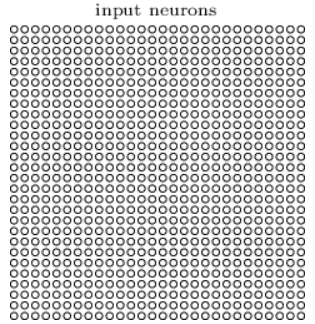
\includegraphics[width=0.5\textwidth]{docu_img_10}
    \caption{Feld von Inputneuronen.}
    \label{fig:field-of-neurons}
\end{figure}

Im Unterschied zu \textit{herkömmlichen} neuronalen Netzen, bei denen üblicherweise alle Input-Neuronen mit allen Neuronen des
nachfolgenden Hidden-Layers verbunden werden, besteht die Besonderheit nun darin, dass jedes Neuron des Hidden-Layers
mit einem kleinen Bereich des Inputs verbunden wird. Dieses Vorgehen kann anhand des folgenden Bildes veranschaulicht
werden:

\begin{figure}[h]
    \centering
    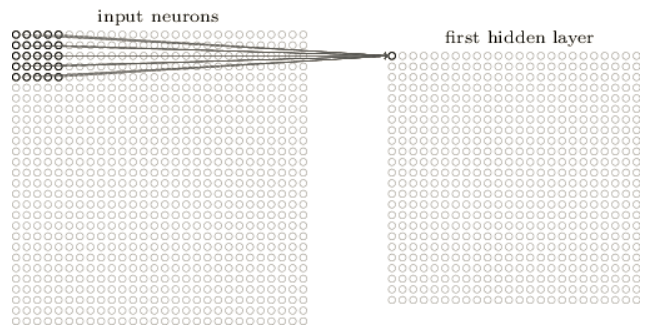
\includegraphics[width=0.9\textwidth]{docu_img_11}
    \caption{Convolution-Prozess, Schritt 1.}
    \label{fig:convolution-process-1}
\end{figure}

Dieses lokale rezeptive Feld wird dann gemäß der Konfiguration über das Input-Bild \textit{bewegt}, so dass alle Input-Neuronen
besucht werden. Demnach sähe der zweite Schritt - unter der Annahme, dass das Feld immer um ein Pixel verschoben wird -
folgendermaßen aus:

\begin{figure}[h]
    \centering
    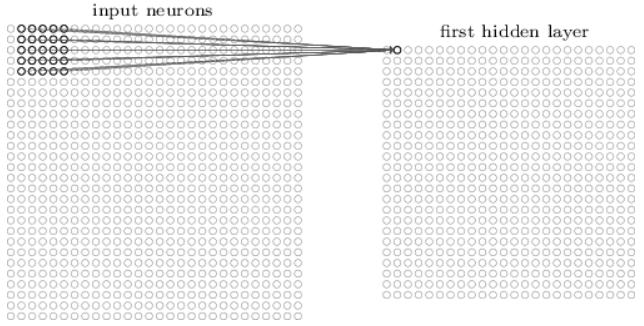
\includegraphics[width=0.9\textwidth]{docu_img_12}
    \caption{Convolution-Prozess, Schritt 2.}
    \label{fig:convolution-process-2}
\end{figure}

Auf diese Art und Weise entsteht das erste Hidden-Layer dessen Größe selbstverständlich etwas kleiner ist, als die Größe
des Input-Layers. Geht man von einem Input-Bild der Größe 28 \(\times\) 28 Pixel und einem lokalen rezeptiven Feld der Größe 5 \(\times\) 5
Pixel aus, so folgt daraus ein erstes Hidden-Layer der Größe 24 \(\times\) 24 Pixel.

\textnormal{\paragraph{Shared Weights}}

Jedes Neuron des Hidden-Layers verfügt wie üblich über einen Bias und - im Falle eines lokalen rezeptiven Felds der
Größe 5 \(\times\) 5 Pixel - über 5 \(\times\) 5 Gewichte. Die Besonderheit besteht nun darin, dass diese Gewichte und Bias für \textit{alle}
Neuronen des Hidden-Layers gleich gelten. Inhaltlich hat dies zur Folge, dass ein konkretes Hidden-Layer genau eine konkrete
\textit{Auffälligkeit} extrahiert. Solch eine konkrete \textit{Auffälligkeit} könnte beispielsweise eine vertikale oder horizontale
Linie sein, die durch die Verwendung des lokalen rezeptiven Felds, das sich über das Bild bewegt, an beliebigen
Positionen aufgespürt werden kann. Üblicherweise reicht es nicht aus, nur eine \textit{Auffälligkeit} aufzuspüren. Aus diesem
Grund besteht ein einziges Layer häufig aus mehreren parallelen Feature Maps.

So könnte ein einziges Hidden-Layer beispielsweise die nachfolgende Form haben, durch das dann drei verschiedene
Auffälligkeiten extrahiert werden würden:

\begin{figure}[h]
    \centering
    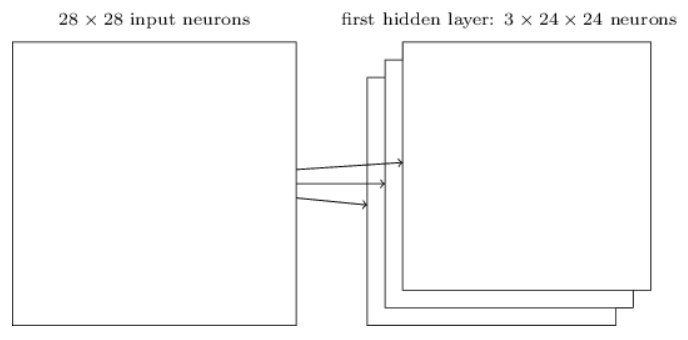
\includegraphics[width=0.9\textwidth]{docu_img_13}
    \caption{Drei Filterschichten.}
    \label{fig:filter-layers}
\end{figure}

Ein weiterer wesentlicher Vorteil bei der Verwendung von \textit{Shared Weights} besteht darin, dass die Anzahl der zu
trainierenden Variablen um ein Vielfaches verringert wird, wodurch ein schnelleres Lernen ermöglicht werden kann.
Eine einzige Feature Map würde bei den bisher betrachteten Dimensionen durch 5 \(\times\) 5 = 25 Gewichte und einen Bias,
also insgesamt 26 Parameter definiert werden. Selbst wenn ein Hidden-Layer aus 20 features maps bestünde, so würde dies
im Ergebnis zu \textit{nur} 20 \(\times\) 26 = 520 Parametern führen.
Wird ein fully connected Layer bestehend aus 30 Neuronen und das gleiche Input-Layer wie zuvor betrachtet, so folgt
daraus, dass insgesamt (28 x 28) x 30 + 30 = 23.550 Parameter in jedem Schritt des Lernens angepasst werden müssen.

\textnormal{\paragraph{Pooling}}

Die zuvor vorgestellten Layer, die durch die Verwendung des lokalen rezeptiven Felds und gemeinsam geteilter Gewichte
enstehen, werden gemeinhin als \textit{convolutional} Layer bezeichnet. Von diesen kann ein weiterer wesentlicher Bestandteil
von convolutional networks abgegrenzt werden - die \textit{pooling} Layer. Diese Art von Layer folgt für
gewöhnlich auf die zuvor vorgestellten \textit{convolutional} Layer und hat zur Aufgabe, die dadurch gewonnenen Informationen
zu vereinfachen.
Das grundsätzliche Vorgehen kann durchaus mit dem des convolutional Layers verglichen werden - auch bei den pooling
Layers kommt ein Feld zum Einsatz, dass sich über das Ergebnis des vorherigen Schrittes bewegt. Es könnte sich
beispielsweise um ein Feld der Größe 2 \(\times\) 2 handeln. Dieses würde somit immer 4 Neuronen betrachten und - im Falle des
max-poolings (einer konkreten Ausprägung des Poolings) - das größte von ihnen auswählen.

Bildlich kann dies auf die folgende Art und Weise veranschaulicht werden:

\begin{figure}[h]
    \centering
    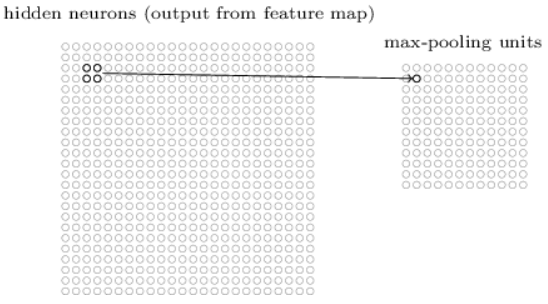
\includegraphics[width=0.9\textwidth]{docu_img_14}
    \caption{Maxpooling Prozess.}
    \label{fig:max-pooling}
\end{figure}

Dadurch, dass vier Neuronen auf ein Neuron projeziert werden, verringert sich die Größe bei diesem konkreten Beispiel
von 24 \(\times\) 24 auf 12 \(\times\) 12. Dieses Vorgehen wird selbstverständlich auf alle feature maps des vorherigen convolutional Layers
angewendet, so dass das folgende Ergebnis entsteht.

\begin{figure}[h]
    \centering
    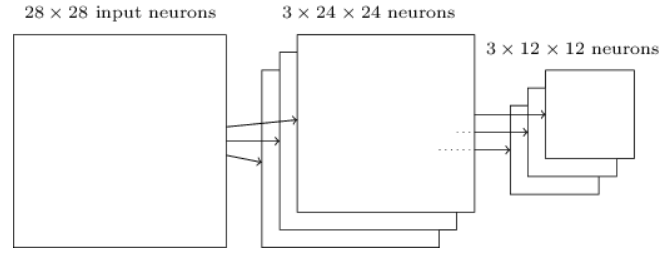
\includegraphics[width=0.9\textwidth]{docu_img_15}
    \caption{Convolution Prozess.}
    \label{fig:convolution-process}
\end{figure}

\subsubsection{Beispielhaftes Convolutional Network}

Nachdem die wesentlichen Bestandteilen eines convolutional Netzes vorgestellt worden sind, können diese nun miteinander
verknüpft werden, um die Architektur eines exemplarischen Netzes zu veranschaulichen. Wie auch bei \textit{normalen} neuronalen
Netzen orientieren sich Input- und Output-Layer an der Struktur des Inputs bzw. Outputs. Dazwischen befinden sich
abwechselnd convolutional und pooling Layer, die grundsätzlich beliebig oft hintereinander geschaltet werden können.
Demnach sähe ein sehr simples convolutional Netzwerk beispielsweise folgendermaßen aus:

\begin{figure}[h]
    \centering
    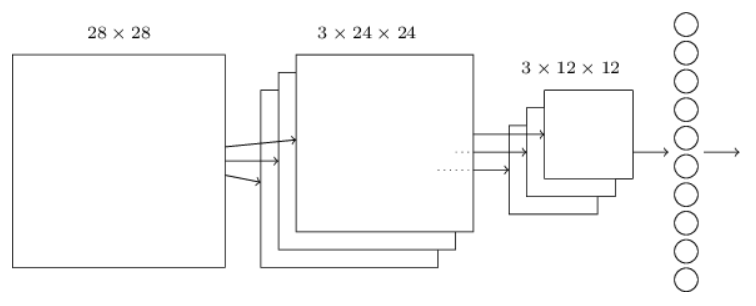
\includegraphics[width=0.9\textwidth]{docu_img_16}
    \caption{Vollständiges \textit{Convolutional Network} mit Klassifizierungs-Ausgabe.}
    \label{fig:convoultional-newtork}
\end{figure}


\section{Frameworks}

Im Umfeld des Machine Learnings sind zahlreiche Frameworks für verschiedene Plattformen und verschiedene Sprachen zu
finden. Diese sind auf unterschiedlichen Abstraktionsebenen angesiedelt und dementsprechend unterschiedlich komplex
in der Verwendung.
Je höher ein Framework dabei angesiedelt, desto einfacher ist es üblicherweise zu bedienen, bietet dem Anwender aber
dafür nur sehr stark eingeschränkte Möglichkeiten. Frameworks hingegen, die auf einem niedrigen Level operieren, bieten
dem Anwender sehr detaillierte und komplexe Möglichkeiten, den gesamtem Programmfluss zu beeinflussen, sind dadurch aber
auch deutlich komplexer zu verwenden.
Die Frameworks sind insbesondere darauf ausgerichtet, eine Implementation für die konkreten mathematischen Berechnungen
und Modelle zu bieten, die darüber hinaus auch hinsichtlich der Performance optimiert worden sind.

Zu nennen wären beispielsweise die nachfolgenden drei Frameworks:

\begin{enumerate}
    \item{Scikit-Learn\footnote{scikit-learn, Machine Learning in Python.\newline(http://scikit-learn.org/stable/)}}
    \item{Keras\footnote{Keras: The Python Deep Learning library.\newline(https://keras.io/)}}
    \item{TensorFlow\footnote{TensorFlow\texttrademark, An open-source machine learning framework for everyone.\newline(https://www.tensorflow.org/)}}
\end{enumerate}

Diese Aufzählung ist nicht vollständig und stellt lediglich einige Repräsentanten dar.

\subsection{Scikit-Learn}

Scikit-Learn stellt einen simplen Einstieg in die Welt des Machine Learnings dar und hält den Großteil der eigentlichen
Komplexität vor dem Anwender verborgen. Scikit-Learn baut im Wesentlichen auf NumPy [http://www.numpy.org/] und
SciPy [https://www.scipy.org/] auf und bietet eine Reihe von einfach zu verwendenden Werkzeugen, die für die Analyse und
Auswertung von Daten genutzt werden können.

\subsection{Keras}

Ähnlich wie Scikit-Learn stellt Keras ebenfalls ein Framework dar, das auf einer verhältnismäßig hohen Ebene operiert.
Die Besonderheit besteht dabei darin, dass Keras eine Schnittstelle zu komplexeren Frameworks wie beispielsweise
TensorFlow oder Theano bereitstellt. Damit eignet Keras sich insbesondere für das schnelle und einfache Entwickeln von
Prototypen.

\subsection{TensorFlow}

Von den beiden zuvor genannten Frameworks kann TensorFlow abgegrenzt werden. TensorFlow bietet eine Reihe von
verschieden komplexen APIs, die dem Anwender Zugang zu verschiedenen Leveln ermöglichen. Die Architektur des Frameworks
kann mit Hilfe der nachfolgenden Grafik verdeutlicht werden:

\begin{figure}[h]
    \centering
    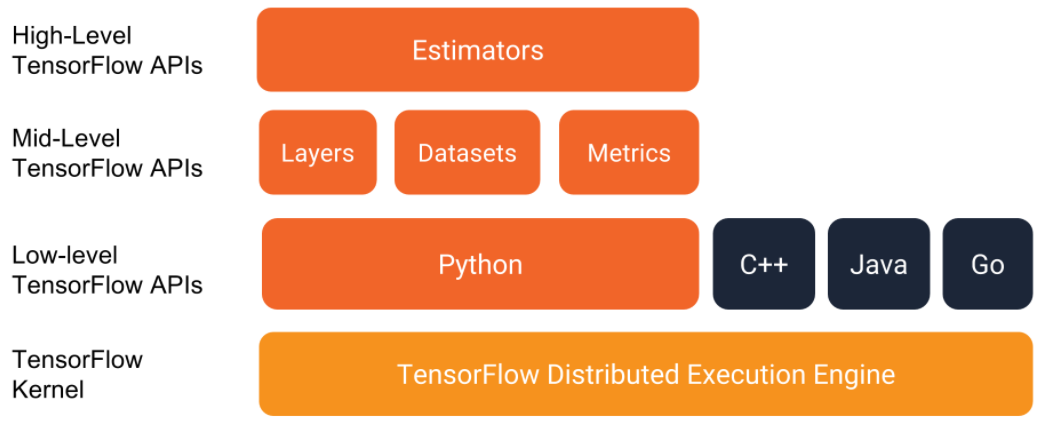
\includegraphics[width=0.9\textwidth]{docu_img_21}
    \caption{Architektur von TensorFlow}
    \label{fig:tf-api}
\end{figure}

Wie Keras und Scikit-Learn bietet auch TensorFlow die Möglichkeit, Verfahren zu verwenden, die leicht zu bedienen sind
und somit keine tiefgehenden Kenntnisse voraussetzen. Darüber hinaus ist es allerdings auch möglich, eigene Modelle und
Strukturen von Grund auf selbst zu definieren und so direkten Einfluss auf das Lernen, Validieren und Vorhersehen zu
nehmen.

\subsubsection{Verwendung von TensorFlow}

In diesem Projekt wurde der Fokus insbesondere auf TensorFlow gelegt. Den elementaren Datentyp von TensorFlow stellen
Tensoren dar. Diese sind mathematisch betrachtet eine Abstraktion von Vektoren und Matritzen. So entspricht ein Tensor
des Typs (0, 0) beispielsweise Skalaren und Tensoren vom Typ (1, 0) Vektoren.
Im Sinne von TensorFlow wird unter einem Tensor\footnote{TensorFlow, tf.Tensor.\newline(https://www.tensorflow.org/api\_docs/python/tf/Tensor)}
ein Platzhalter für den Output einer Operation\footnote{TensorFlow, tf.Operation.\newline(https://www.tensorflow.org/api\_docs/python/tf/Operation)} verstanden.
Die Besonderheit besteht dabei darin, dass ein Tensor lediglich einen Platzhalter darstellt und keine konkreten Werte
repräsentiert. Der Tensor repräsentiert vielmehr eine Berechnungsvorschrift, nach der sein Output zu berechnen ist.
Auf diese Art und Weise können mehrere Operationen miteinander verkettet werden, die jeweils einen Tensor als Input und
Output haben. Dadurch entsteht ein Graph\footnote{TensorFlow, tf.Graph.\newline(https://www.tensorflow.org/api\_docs/python/tf/Graph)},
der demnach eine komplette Berechnung repräsentiert. Sobald diese Berechnung im Rahmen einer Session\footnote{TensorFlow, tf.Session.\newline(https://www.tensorflow.org/api\_docs/python/tf/Session)}
ausgeführt wird, \textit{fließt} der Input durch den zuvor definierten Graphen, so dass schlussendlich ein Output
produziert wird.

TensorFlow macht demnach starken Gebrauch des \textit{DataFlow-Paradigmas}\footnote{Wikipedia, Dataflow programming.\newline(https://en.wikipedia.org/wiki/Dataflow\_programming)},
wodurch insbesondere die Parallelisierung von Berechnungen erheblich begünstigt wird.

Das Zusammenspiel von Graphen und Sessions kann anhand der nachfolgenden Graphik verdeutlicht werden:

\begin{figure}[H]
    \centering
    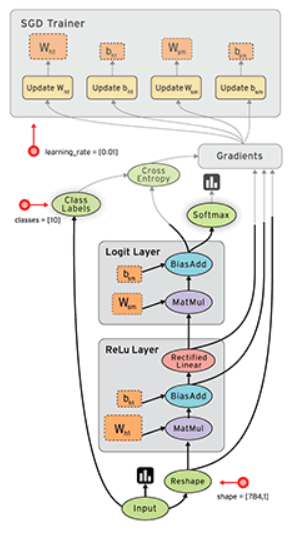
\includegraphics[width=0.5\textwidth]{docu_img_22}
    \caption{Exemplarischer \textit{Dataflow}.}
    \label{fig:tf-api}
\end{figure}
\par
Da im Rahmen des Projekts auf einige Probleme bei der Verwendung von TensorFlow gestoßen wurde, wurde parallel zum
Betrieb von TensorFlow versucht, das Modell mit Keras nachzubauen. Keras ist etwas abstrakter als TensorFlow und bietet
dem Anwender so weniger Konfigurationsmöglichkeiten, wodurch andererseits auch eigene Fehler ausgeschlossen oder eliminiert
werden können.



\section{Bericht, Meilensteine und Ziele des Projekts}

Nachfolgend soll dem Leser ein Einblick in den Ablauf des Projekts gewährt werden. Dabei soll auf Meilensteine, die im
Vorfeld definiert worden sind, eingegangen werden, Probleme thematisiert werden, die während der Durchführung aufgetreten
sind, Anpassungen und Änderungen, die im Zuge des Auftretens von Problemen vorgenommen werden mussten, dargelegt werden
und schlussendlich auch Erkenntnisse, die durch die Durchführung des Projekts gesammelt werden konnten, aufgezeigt werden.

Das thematische Ziel (die möglichst gute Wiederherstellung von unkenntlich gemachten Gesichtern) wurde bereits an anderer
Stelle umfangreich thematisiert.

Neben dem inhaltlichen Ziel galt es auch insbesondere tiefgehende Kenntnisse über das Machine Learning zu erlangen.
Dabei handelte es sich zum einen um die theoretische Seite, die sich zusammensetzte aus den grundlegenden Prinzipien des
Machine Learnings, neuronalen Netzen und ganz konkreten Convolutional Networks, und zum anderen um die eher praktische
Seite, die durch die Verwendung des Frameworks TensorFlow charakterisiert wurde.

Im Vorfeld wurden insbesondere die nachfolgenden wesentlichen Meilensteine festgelegt:

\begin{enumerate}
    \item{Verschaffen eines Überblicks über den State of the Art und vergleichbare Projekte und Forschungsarbeiten}
    \item{Beschaffung von entsprechenden Daten und deren Aufbereitung}
    \item{Erlangung von theoretischen Kenntnissen über neuronale Netze (insbesondere Convolutional Networks)}
    \item{Modellierung eines Convolutional Networks}
    \item{Umsetzung des zuvor definierten Modells in TensorFlow (und anderen Frameworks)}
    \item{Trainieren des Netzes}
    \item{Produzieren von brauchbaren Ergebnissen}
\end{enumerate}

\subsection{Verschaffen eines Überblicks über den State of the Art}

Das Thema Machine Learning erfährt derzeit einen unfassbar großen Hype. Infolgedessen finden sich viele verschiedene
Forschungsarbeiten und Projekte, die sich mit der Verarbeitung von Bildern beschäftigen. Insbesondere fällt dabei auf,
dass die Qualität des Ergebnisses maßgeblich von der Qualität und insbesondere auch der Masse der Traininsdaten abhängt.
Projekte, die sich mit vergleichbaren Thematiken befassten, haben beispielsweise mit mehreren hunderttausend Datensätzen
trainiert. Die Anzahl der in diesem Projekt verwendeten Datensätze beläuft sich auf etwa knapp 2.500 Bilder, was
offensichtlich eine deutlich kleinere Größenordnung ist.
Ein weiterer entscheidender Parameter ist die Anzahl der Epochen. Eine Epoche meint dabei, dass jeder Datensatz der
Trainingsdaten einmal betrachtet worden ist. Durch eine Erhöhung der Anzahl der Epochen ist es möglich, das zu trainierende
Modell präziser auf die Daten abzustimmen - dabei gilt es jedoch zu beachten, dass zu viele Epochen dazu führen können,
dass es zum \textit{Overfitting} kommt und das Modell ``zu gut'' an die Traininsdaten angepasst wird, so dass
über unbekannte Datensätze deutlich fehlerbehaftete Aussagen getroffen werden können.

\subsection{Beschaffung von entsprechenden Daten und deren Aufbereitung}

Da die Daten, wie im vorherigen Absatz beschrieben, einen elementaren Anteil zur Qualität des Ergebnisses leisten, galt
es im ersten Schritt zunächst, diese zu erlangen und entsprechend aufzubereiten. Unter der Aufbereitung der Daten wird
dabei zum einen verstanden, diese zu vereinheitlichen, und zum anderen, sie so anzupassen, dass das Modell mit ihnen
effektiv trainiert werden kann. Aus diesem Grund wurde sich beispielsweise dazu entschieden, die Bilder auf eine Größe
von 64 x 96 Pixel zu reduzieren und sie auf einen Farbkanal zu reduzieren, so dass Graustufen-Bilder entstehen, um so
die Trainingsdauer deutlich verringern zu können.

\subsection{Erlangung von theoretischen Kenntnissen}

Wie bereits eingangs erwähnt stand neben dem inhaltlichen Ziel auch der Aufbau von neuem Wissen im Vordergrund. Durch die
intensive Auseinandersetzung mit verschiedensten Forschungsarbeiten aus dem Bereich des Machine Learnings im Kontext der
Verarbeitung von Bildern sowie dem Bearbeiten von Literatur, konnte ein tiefergehendes Verständnis für die grundlegenden
Prinzipien des Machine Learnings und insbesondere auch neuronale Netze erlangt werden.
Darüber hinaus konnten auch Erfahrungen im Umgang mit weit verbreiteten Frameworks, die im wissenschaftlichen Bereich und
in der Bildverarbeitung verwendet werden, gesammelt werden. Dazu zählt insbesondere NumPy\footnote{NumPy, NumPy.\newline(http://www.numpy.org/)}.
Da im Rahmen der Veranstaltung ``Soft Computing'' bereits erste Berührungspunkte verzeichnet werden konnten, bestand der
Wunsch dies noch zu vertiefen und sich auf einer niedrigeren Ebene mit den Thematiken zu befassen. Aus diesem Grund wurde
TensorFlow als Unterstützung gewählt, das dem Anwender tiefere Einblicke gewährt, als es beispielsweise bei Scikit-Learn
der Fall ist.

\subsection{Modellierung eines Convolutional Networks}

Eine spannende Phase stellte die Modellierung des Convolutional Networks, das für die Verarbeitung der Bilder benutzt
werden sollte, dar. Dabei galt es, die theoretischen Kenntnisse, die im Kapitel \textit{Neuronale Netze} genauer
beschrieben werden, anzuwenden und durch eine entsprechende Kombination der verschiedenen Arten von Layern ein Modell
zu entwickeln, in das die zuvor beschafften Daten eingespeist werden können.

\subsection{Umsetzung des zuvor definierten Modells in TensorFlow}

Dieser Meilenstein und der zuvor genannte fanden größtenteils parallel statt, da die theoretischen Überlegungen zumeist
umgehend umgesetzt wurden, um deren Praktikabilität beurteilen zu können. Die Umsetzung des Modells stellte dabei nur
einen Teil der gesamten Umsetzung dar. Darüber hinaus musste zunächst ein entsprechender Rahmen geschaffen werden, in
dem das Modell Verwendung finden konnte. Dies kann anhand des Repositorys nachvollzogen werden.

\subsection{Trainieren des Netzes}

Einen zentralen Bestandteil des Machine Learnings stellt selbstverständlich das Trainieren des entwickelten Modells dar.
Die Schwierigkeit besteht dabei darin, dass der Lernvorgang je nach Größe, Komplexität und Umfang der Daten eine gewisse
Zeitdauer erfordert. Konkret bedeutet das, dass eine Epoche bei einem Training des Modells mit knapp 2.500 Bildern mitunter
2 Stunden Zeit in Anspruch genommen hat. Infolgedessen war es schwierig und zugleich zeitaufwendig zu beurteilen,
inwieweit Änderungen an dem Modell und den Parametern, die dieses beeinflussen, zu Verbesserungen oder Verschlechterungen
führten.

\subsection{Produzieren von brauchbaren Ergebnissen}

Zum einen stellt der Ansatz des Machine Learnings durchaus einen faszinierenden Ansatz dar, da ohne konkrete Nennung von
Regeln und Anweisungen, ein System geschaffen wird, das in der Lage ist, Aussagen über bekannte sowie unbekannte Daten
treffen zu können. Damit einher geht allerdings auch eine gewisse Problematik, die bei Convolutional Networks und auch
anderen Methodiken des Machine Learnings, die eine entsprechende Größe und Komplexität haben, auftritt. Es ist mitunter
schwierig nachzuvollziehen, was sich hinter den konkreten Gewichten und Anpassungen des Systems verbirgt. Dies erschwert
die Suche nach Fehlern und das Debugging immens.
Auf der einen Seite stellt das Verwenden von Frameworks wie beispielsweise TensorFlow oder Scikit-Learn eine Hilfestellung
dar, die dem Anwender ermöglicht, sich auf die konkreten inhaltlichen Problematiken konzentrieren zu können. Auf der
anderen Seite bleibt dem Anwender dadurch ein großer Teil der darunterliegenden Komplexität verborgen. Dies stellt
selbstverständlich je nach Betrachtungswinkel auch einen Vorteil dar. Sobald allerdings Ergebnisse entstehen, die nicht
dem Erwarteten entsprechen, kann es sich als durchaus schwierig herausstellen, die Ursachen dafür aufzuspüren.

Nachfolgend werden die mit Keras erzielten Ergebnisse aufgelistet. Dabei repräsentiert die ersten Spalte den Input,
die darauffolgenden drei Spalten die Ergebnisse nach der ersten, fünften und zehnten Epoche und die letzte Spalte das
Originalbild, das nach Möglichkeit wiederhergestellt werden sollte.

\begin{figure}[!htb]
    \begin{adjustwidth}{-2cm}{}
        \captionof{table}{Mit \textit{Keras} erzielte Resultate.}
        \begin{tabular}{ c | c | c | c | c }
            \small{Input} & \small{1. Epoche} & \small{5. Epoche} & \small{10. Epoche} & \small{Original} \\
        \hline
            
\includegraphics[width=0.2\textwidth]{blur_03_in} &
            
\includegraphics[width=0.2\textwidth]{blur_03_ep_1} &
            
\includegraphics[width=0.2\textwidth]{blur_03_ep_5} &
            
\includegraphics[width=0.2\textwidth]{blur_03_ep_10} &
            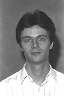
\includegraphics[width=0.2\textwidth]{96_64_target} \\
        \hline
            
\includegraphics[width=0.2\textwidth]{mosaic_05_in} &
            
\includegraphics[width=0.2\textwidth]{mosaic_05_ep_1} &
            
\includegraphics[width=0.2\textwidth]{mosaic_05_ep_5} &
            
\includegraphics[width=0.2\textwidth]{mosaic_05_ep_10} &
            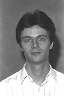
\includegraphics[width=0.2\textwidth]{96_64_target} \\
        \end{tabular}
    \end{adjustwidth}
\end{figure}

\clearpage


\section{Fazit}

Die Ergebnisse, die dieses Projekt liefert, sind von einem verwendbaren Resultat noch etwas entfernt. Dennoch sieht man eine
valide Approximation, die auch nach zehn Epochen noch nicht abgeschlossen zu sein scheint. Wir sind der Überzeugung, dass die Resultate,
mit Anpassungen folgender Parameter, durchaus brauchbar werden können.

\subsection{Trainingsdatensätze}
Ideal wäre eine Datenbank ähnlich der \textit{FaceScrub}\textsuperscript{\ref{footnote:face-scrub}} jedoch mit mehr
individuellen Personen in natürlicher Umgebung. Denn soll das Netz dazu verwendet werden, Bilder widerherzustellen, so
besteht dort kein Einfluss auf den Kontext, in dem das Ursprungsbild aufgenommen wurde.
Zudem sollte es sich als hilfreich erweisen, Bilder in einer möglichst großen Auflösung zum Trainieren zu verwenden, da
eine Vergrößerung der Urspungsbilder verlustfrei möglich ist. Muss das Ursprungsbild jedoch zuvor runterskaliert werden, geht
an dieser Stelle schon Information verloren, die sonst dazu dienen könnte, eine mögliche Ursprungsinformation wiederherzustellen.

\subsection{Lerndauer}
Das Netz noch mehr zu trainieren war, mit den uns zur Verfügung stehenden Computern, nicht möglich. Eine unterstüzende Maßnahme
hierfür könnte \textit{Cloud Computing}\footnote{Wikipedia, Cloud Computing.\newline(https://de.wikipedia.org/wiki/Cloud\_Computing)}
sein, mit der es möglich wäre noch mehr Datensätze in einer noch kürzeren Zeit zu lernen.


\newpage

\listoffigures % Print the list of figures

\listoftables % Print the list of tables

%----------------------------------------------------------------------------------------
%	BIBLIOGRAPHY
%----------------------------------------------------------------------------------------

\renewcommand{\refname}{\spacedlowsmallcaps{References}} % For modifying the bibliography heading

\bibliographystyle{unsrt}

\bibliography{sample.bib} % The file containing the bibliography

%----------------------------------------------------------------------------------------

\end{document}